\documentclass{article}
\usepackage{hyperref}
\usepackage{enumitem}
\usepackage{graphicx}

\begin{document}
\title{Technical Paper Proposal: \\ Placement Algorithms for Heterogenous FPGAs}
\author{Brian B Cheng \\ Department of Electrical and Computer Engineering}


\date{}
\maketitle

\section{Proposal}
In the software world, an engineer writes a program in a high-level langauge like C, Java, or Python. 
Then the engineer compiles the program using some compilation software like gcc or clang. 
First, the compiler takes the engineer's high-level program, and through multiple stages of lexing, parsing, and optimizations, generates a low-level program in an assembly language like x86 or MIPS. 
Then, the compiler assembles the assembly code into machine code. 
The produced machine code is often referred to as a binary and is ready to execute on the machine. 
Different compilers may have different strategies for this process. 
For example, LLVM and clang skip the assembly stage and go directly from high-level code to machine code, while gcc sticks to the traditional two-step process. 
The Java and Python are more complex in that they compile high-level code into an intermediate language as bytecode. 
In Java, the compiler assembles the bytecode into machine code at runtime in a process called Just-in-Time compilation which allows it to be platform independent. 
Python offers the choice to assemble the machine code before or at runtime. 
Simplify this downto 2 sentences.


In the FPGA world, the design entry to product pipeline is despairingly complex by comparison. First, the design entry. The engineer describes a digital system using a high-level HDL like Verilog or VHDL. Then the engineer submits the design entry to an EDA like Vivado or Quartus to perform three stages of automated design. These are: synthesis, placement, and routing. and then yap about NP-hardness and massive search space and hellish runtime.


\section{Abbreviations}
\begin{itemize}[label={--}, left=0.25cm] % Adjust label and left indent as desired
    \item \textbf{FPGA}: Field Programmable Gate Array
    \item \textbf{VLSI}: Very Large Scale Integration
    \item \textbf{EDA}: Electronic Design Automation
    \item \textbf{VHSIC}: Very High Speed Integrated Circuits
    \item \textbf{HDL}: Hardware Description Language
    \item \textbf{VHDL}: VHSIC HDL
    \item \textbf{HLS}: High Level Synthesis: Generating synthesizable HDL from high-level software languages. A company might want to have a software engineer write C or C++ code and have a program translate it into synthesizable Verilog. This can can boost productivity and save the company the need to hire a hardware engineer.
    \item \textbf{IP}: Intellectual Property: In FPGA context, this means pre-built modules or subsystems like a hardened microprocessor or Ethernet controller. These are usually proprietary.
    \item \textbf{SoC}: System on Chip: An FPGA device (chip) that features hardened IP in addition to the programmable logic fabric.
    \item \textbf{PL-PS}: Programmable Logic - Processing System: A design that utilizes the on-chip hard microprocessor in conjunction with the programmable logic fabric.
    \item \textbf{EDIF}: Electronic Design Interchange Format
    \item \textbf{HPWL}: Half Perimeter Wire Length
\end{itemize}

\section{Keywords}
\begin{itemize}
    \item FPGA, EDA, Synthesis, Placement, Routing, Parallel, Optimization
\end{itemize}

\section{Ideas}
\begin{itemize}[label={\textbullet}, left=0.25cm]
    \item \textbf{FPGA}: Field Programmable Gate Array
    \begin{itemize}[label={--}, left=0.25cm]
        \item FPGA Vendors:
        \begin{itemize}[label={$\cdot$}, left=0.25cm]
            \item AMD-Xilinx ($\sim$50\% FPGA vendor market share)
            \item Intel-Altera ($\sim$35\% share)
            \item Lattice
            \item Microsemi
        \end{itemize}
    \end{itemize}

    \item \textbf{EDA}: Electronic Design Automation
    \begin{itemize}[label={--}, left=0.25cm]
        \item Proprietary software for FPGA and VLSI development:
        \begin{itemize}[label={$\cdot$}, left=0.25cm]
            \item Xilinx - Vivado (Design + Simulation) + Vitis (HLS + PL-PS codesign)
            \item Altera - Quartus (Design) + ModelSim (Simulation)
            \item Synopsis (VLSI)
            \item Cadence (VLSI)
        \end{itemize}
        \item Open source software for FPGA development:
        \begin{itemize}[label={$\cdot$}, left=0.25cm]
            \item \textbf{VTR}: Simulated Annealing placer for FPGAs. Popular among researchers who study placement techniques. Commonly referred to as an "academic placer".
            \item \textbf{OSS-CAD}: a full-flow software suite that includes ABC synthesis, Yosys synthesis, Yosys nextpnr.
            \item \textbf{AMF-Placer}: Analytical Placer for FPGAs
            \item \textbf{RapidWright}: Semi-open source API that provides backend access to Xilinx Vivado EDA using design checkpoints.
            \item \textbf{RapidLayout}: Hard Block Placer for Systolic Arrays. Built with RapidWright.
            \item \textbf{RapidStream}: HLS Placer. Built with RapidWright.
            \item \textbf{DREAMPlace}: GPU-powered deep learning placement for VLSI.
            \item \textbf{DREAMPlaceFPGA}: DREAMPlace, adapted to FPGAs via the RapidWright API.
        \end{itemize}
    \end{itemize}
    
    \item \textbf{Synthesis}
    \begin{itemize}[label={--}, left=0.25cm]
        \item Takes a design written in a high-level HDL like VHDL or Verilog and "synthesizes" a \textbf{logical netlist} out of it. 
        \item The logical netlist is usually generated as an EDIF, JSON, or a low-level Verilog file. 
        \item The netlist describes the necessary basic elements of logic (BELs) and the wired connections between them that are necessary to implement the design.
    \end{itemize}

    \item \textbf{Placement}
    \begin{itemize}[label={--}, left=0.25cm]
        \item Takes the \textbf{logical netlist} and produces a \textbf{physical netlist}.
        \item For each BEL in the netlist, assign the BEL to a Cell, Site, and Tile on the physical FPGA device.
    \end{itemize}

    \item \textbf{Routing}
    \begin{itemize}[label={--}, left=0.25cm]
        \item Takes the \textbf{physical netlist} and maps the connections between BELs onto wires, interconnects, and switchboxes on the FPGA.
    \end{itemize}

\end{itemize}

\newpage
\begin{figure}
    \begin{center}
        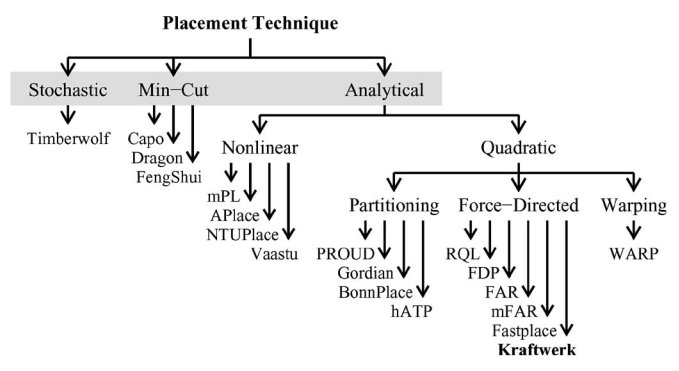
\includegraphics[width=0.75\textwidth]{figures/kraftwerk2.png}
    \end{center}
    \caption{Landscape of VLSI placement techniques (Spindler) \cite{kraftwerk2} }
    \label{fig:kraftwerk2}
\end{figure}
\begin{figure}
    \begin{center}
        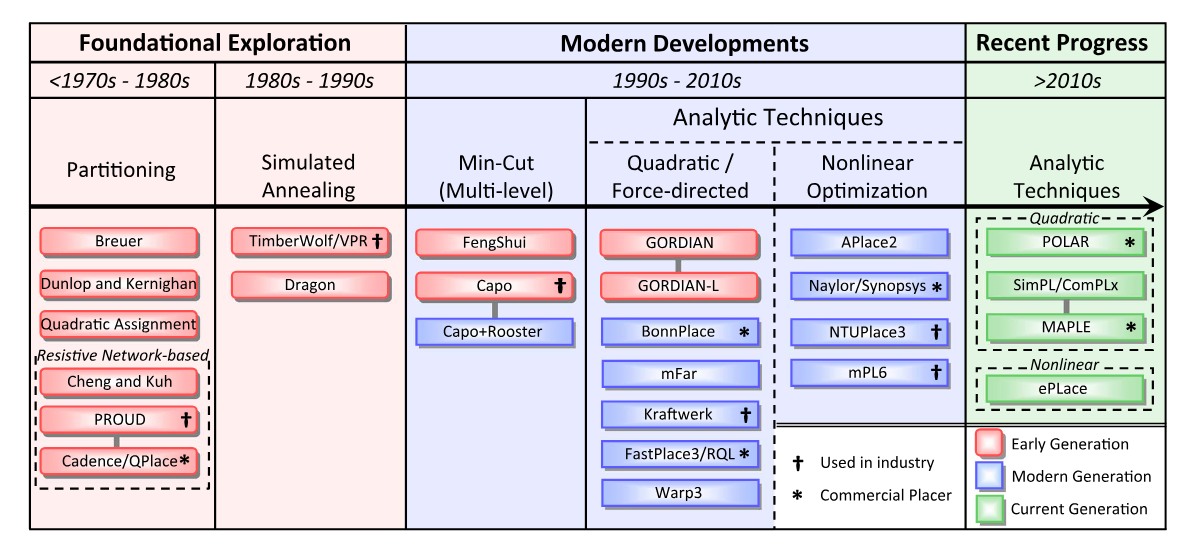
\includegraphics[width=0.95\textwidth]{figures/ProCha.png}
    \end{center}
    \caption{Historical timeline of VLSI placement techniques (Markov) \cite{ProCha} }
    \label{fig:ProCha}
\end{figure}

This is a citation for AMFPlacer. \cite{AMFPlacer}

\newpage
\bibliographystyle{ieeetr}
\nocite{*}
\bibliography{
    references/surveys,
    references/rapidwright,
    references/fpga_placement,
    references/vlsi_placement,
}

\end{document}


